% Feel free to contact me for any reason:
%% Email 1: zain.kamal@rutgers.edu
%% Email 2: z.kamal2021@gmail.com
%% Discord: alci#6038

%%%%%%%%%%%%%%%%%%%%%%%%%%%%%%%%%%%%%%%%%%%%%%%%%%%%%%%%%%%%%%%%%%%%%%%%%%%%%%%%%
\documentclass{article}
% Feel free to contact me for any reason:
%% Email 1: zain.kamal@rutgers.edu
%% Email 2: z.kamal2021@gmail.com
%% Discord: alci#6038

% Last updated 1/28/22

% Template based off of Justin Kim's (don't know where he got it from originally), but I've made a ton of edits. His soul lives on in random packages and commands I'm too lazy to comment out.


%%%%%%%%%%%%%%%%%%%%%%%%%%%%%%%%%%%%%%%%%%%%%%%%%%%%%%%%%%%%%%%%%%%%%%%%%%%%%%%%%%%%
%%% Default packages:

\usepackage[margin=1in]{geometry} 
\usepackage{amsmath,amsthm,amssymb,amsfonts, fancyhdr, color, comment, graphicx, environ}
\usepackage{xcolor}
\usepackage{mdframed}
\usepackage{bm}
\usepackage[shortlabels]{enumitem}
\usepackage{mathtools}
\usepackage{listings}
\usepackage{stmaryrd}
\usepackage{indentfirst}
\usepackage{hyperref}


%%%%%%%%%%%%%%%%%%%%%%%%%%%%%%%%%%%%%%%%%
%%% Pacakages I've added:

%% For Math 300 (Winter 2021):

\usepackage{mathdots} % for \iddots

\usepackage[ruled]{algorithm2e} % Algorithms
% NOTE: FIND A BETTER ALGORITHM PACKAGE, OR ATLEAST LEARN HOW TO USE THIS ONE BECAUSE DOUBLE INDENTING IS A FUCKING NIGHTMARE (or just import from mathcha?)
%% Example algorithm:
% \begin{center}
% 	\begin{minipage}{0.5\linewidth} % Adjust the minipage width to accomodate for the length of algorithm lines
% 		\begin{algorithm}[H]
% 			\KwIn{$(a, b)$, two floating-point numbers}  % Algorithm inputs
% 			\KwResult{$(c, d)$, such that $a+b = c + d$} % Algorithm outputs/results
% 			\medskip
% 			\If{$\vert b\vert > \vert a\vert$}{
% 				exchange $a$ and $b$ \;
% 			}
% 			$c \leftarrow a + b$ \;
% 			$z \leftarrow c - a$ \;
% 			$d \leftarrow b - z$ \;
% 			{\bf return} $(c,d)$ \;
% 			\caption{\texttt{FastTwoSum}} % Algorithm name
% 			\label{alg:fastTwoSum}   % optional label to refer to
% 		\end{algorithm}
% 	\end{minipage}
% \end{center}



%%%%%%%%%%%%%%%%%%%%%%%%%%%%%%%%%%%%%%%%%%%%%%%%%%%%%%%%%%%%%%%%%%%%%%%%%%%%%%%%%%%%
%%% Default commands:

\renewcommand{\vec}[1]{\mathbf{#1}}
	
\newcommand{\WidestEntry}{$lon_1$}%
\newcommand{\SetToWidest}[1]{\makebox[\widthof{\WidestEntry}]{#1}}%
\newcommand\tab[1][0.61cm]{\hspace*{#1}}
\newcommand{\nats}{\mathbb{N}}
\newcommand{\rats}{\mathbb{Q}}
\newcommand{\reals}{\mathbb{R}}
\newcommand{\Z}[1]{\mathbb{Z}_{#1}}
\newcommand{\BigO}[1]{\mathcal{O}(#1)}
\newcommand{\seq[1]}{(#1_n)}
\newcommand{\subseq[1]}{(#1_{n_k})}
\newcommand{\Lim}[2]{\lim \limits _{#1 \to #2}}
\newcommand{\Min}[2]{\min \{#1, #2\}}
\newcommand{\inv}{^{-1}}
\newcommand{\h}{^\text{th}}
\newcommand{\lrangle}[1]{\langle #1 \rangle}
\newcommand{\abs}[1]{\left\lvert #1 \right\rvert}

\DeclarePairedDelimiter{\ceil}{\lceil}{\rceil}
\DeclarePairedDelimiter{\floor}{\lfloor}{\rfloor}
\DeclareMathOperator{\supp}{supp}
\DeclareMathOperator{\rad}{rad}
\DeclareMathOperator*{\argmin}{arg\,min}
\DeclareMathOperator*{\argmax}{arg\,max}
\DeclareMathOperator*{\Var}{Var}
\DeclareMathOperator*{\Cov}{Cov}
\DeclareMathOperator*{\Corr}{Corr}
\DeclareMathOperator*{\Aut}{Aut}
\newcommand{\prob}[1]{\section*{Problem #1}}


%%%%%%%%%%%%%%%%%%%%%%%%%%%%%%%%%%%%%%%%%
%%% Commands I've added:

%% For Math 300 (Winter 2021):

\newcommand{\lrbrace}[1]{\{ #1 \}}
\newcommand{\powerset}{\mathcal{P}}
\newcommand{\ints}{\mathbb{Z}}

% Source/inspiration: https://tex.stackexchange.com/a/42728:
\newcommand{\numberthis}{\addtocounter{equation}{1}\tag{\theequation}\label{\theequation}}
    % Within an `align*` environment, put `\numberthis` after a line to number it. 
    % Access it with `\eqref{ [number of equation] }`
\newcommand{\numberthiswith}[1]{\addtocounter{equation}{1}\tag{\theequation}\label{#1}}
    % Within an `align*` environment, put `\numberthiswith{ [your_label] }` after a line to number it. 
    % Access it with `\eqref{ [your_label] }`



%%%%%%%%%%%%%%%%%%%%%%%%%%%%%%%%%%%%%%%%%%%%%%%%%%%%%%%%%%%%%%%%%%%%%%%%%%%%%%%%%%%%
%%% Default formatting:

\hypersetup{
    colorlinks=true,
    linkcolor=blue,
    filecolor=magenta,      
    urlcolor=blue,
}

\setlength{\parindent}{0cm}
\setlength{\parskip}{6pt}

\pagestyle{fancy}


%% Misc formatting additions

% make bullets with itemize much smaller
\newlength{\mylen}
\setbox1=\hbox{$\bullet$}\setbox2=\hbox{\tiny$\bullet$}
\setlength{\mylen}{\dimexpr0.5\ht1-0.5\ht2}
\renewcommand\labelitemi{\raisebox{\mylen}{\tiny$\bullet$}}


% Modified version of problem environment below
% \newenvironment{problem}[2][Problem]
%     { \begin{mdframed}[backgroundcolor=gray!5] \textbf{#1 #2} \\}
%     {  \end{mdframed}}
% \newenvironment{solution}{\textbf{Solution}\\}


%%%%%%%%%%%%%%%%%%%%%%%%%%%%%%%%%%%%%%%%%
%%% Formatting I've added:

%% Grey boxes for problem statements (note that I don't have a "solution" section):

% Problem environment, but shows "(a)" instead of "Problem a"
\newenvironment{problem}[2][]
    { \begin{mdframed}[backgroundcolor=gray!5] \textbf{#1 (#2)}}
    {  \end{mdframed}}
% Problem environment, but no "([input_char])" at all
\newenvironment{problem*}
    { \begin{mdframed}[backgroundcolor=gray!5] \\}
    {  \end{mdframed}}


% Example environment, currently identical to "problem" (Note: this is better written than the problem environment because I wrote it myself from scratch. Use this as an example for future new environments.)
\newcounter{example}[section]
\newenvironment{example}
    { 
        \refstepcounter{example}
        \begin{mdframed}[backgroundcolor=gray!5]
        \textbf{\\Example \thesection.\theexample:}
    }
    {\\ \end{mdframed}}


%%%%%%%%%%%%%%%%%%%%%%%%%%%%%%%%%%%%%%%%%%%%%%%%%%%%%%%%%%%%%%%%%%%%%%%%%%%%%%%%%%%%
% Misc things I've added




%%%%%%%%%%%%%%%%%%%%%%%%%%%%%%%%%%%%%%%%%%%%%
% Fill in the appropriate information below
\lhead{Zain Kamal}
% \rhead{Math 244 Spring 2022} % Moved to document
% \chead{\textbf{Homework 2}} % Moved to document
\begin{document}
\chead{\textbf{Math 244: Lecture Notes 2}}
\rhead{1/20/22}
%%%%%%%%%%%%%%%%%%%%%%%%%%%%%%%%%%%%%%%%%%%%%%%%%%%%%%%%%%%%%%%%%%%%%%%%%%%%%%%%%


\section{Slope Fields}

Given a family of functions representing the solutions to an ODE, we can visualize the differential equation itself as a slope field that describes the ``flow" (tangent vectors) in $\mathbb{R}^{2}$. 


For example, consider the first order ODE $y'=t$ with the solution $y=\tfrac{1}{2} t^{2} +C$:

\begin{figure}[htp]
    \centering
    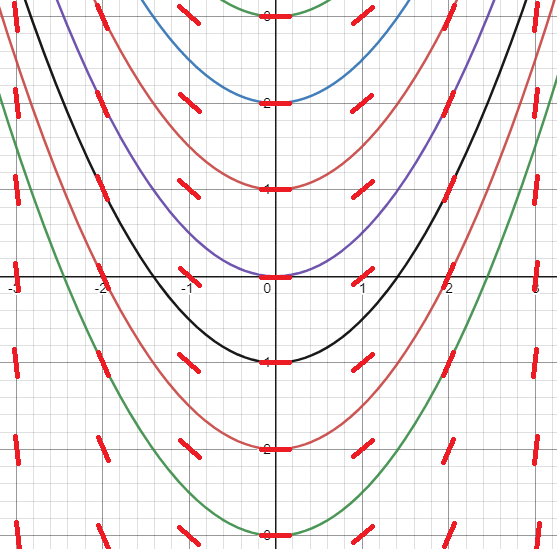
\includegraphics[width=4cm]{images/slope fields.png}
\end{figure}

\
\hline
\section{Separable ODEs}

Recall that the explicit form of first-order (linear) ODEs is:
\begin{equation*}
y'=f( t,y) .
\end{equation*}


Similarly, \underline{separable ODEs} take the explicit form:
\begin{equation}
\boxed{y'=g( t) \ h( y)} .
\end{equation}
Note that the obvious implication of this is that not all first-order ODEs are separable.


\subsection{Nonlinear Separable ODEs (Procedure to Solve)}

Note that if $h( y_{0}) =0$, then $y_{0}$ is a solution of (1): the RHS is forced to be 0, and the LHS is 0 because the derivative of a constant ($y_{0}$) is 0. 



To find \textbf{non-constant} solutions, we take a similar approach to section 2.1 in Lecture Notes 1, and rewrite (1):
\begin{align*}
\frac{dy}{dt} & =g( t) \ h( y)\\
\int \frac{dy}{h( y)} & =\int g( t) \ dt\\
a( y) & =b( t) . \numberthis
\end{align*}
This is called the \underline{implicit solution}, which effectively eliminates the derivative in favor of arbitrary functions in terms of $y$ and $t$. Finally, we can solve for some $y=y( t)$.

\

\textbf{Note 2.1.A:} If we're given some \underline{IVP} (initial value proposition $y( t_{0}) =y_{0}$), we can fully define our general solution (ie find a value of $C$),,,

Be sure to define an interval for the domain of $t$ to avoid indeterminate solutions (eg div by 0). The interval \textbf{must} be ``connected'' to the IVP (see 2.1.2). [WHY THE FUCK??? ASK IN RECITATION]

\begin{example}

\textit{Problem:} Solve $y'=t^{2} y^{2}$. 

\textit{Solution:}

$y'$ is \textit{separable}, with $\begin{cases}
g( t) =t^{2}\\
h( y) =y^{2}
\end{cases}$.



To find \textit{constant solutions}, let $h( y) =y^{2} =0$. Thus $y=0$.



For \textit{general solutions} ($y\neq 0$), find the implicit form:
\begin{align*}
\int \frac{dy}{y^{2}} & =\int t^{2} \ dt\\
\frac{-1}{y} & =\frac{t^{3}}{3} +C_{1}\\
\Longrightarrow y & =\frac{-3}{t^{3} +C} .
\end{align*}
Thus, $y_{gen} =\left\{0,\ \frac{-3}{t^{3} +C}\right\}$.

\end{example}
\

\begin{example}

\textit{Problem:} 
$\begin{cases}
y'=( 1-2x) y^{2}\\
y( 0) =\tfrac{-1}{6}
\end{cases}$

\textit{Solution:}

For $y\neq 0$,
\begin{align*}
\int \tfrac{dy}{y^{2}} & =\int ( 1-2x) \ dx\\
y & =\frac{-1}{x-x^{2} +C} .
\end{align*}
Our IVP implies $C=6$. Thus $y( x) =\frac{1}{( x-3)( x+2)}$.



Since $x\neq 3$ and $x\neq -2$, we may naively conclude that the domain of $y$ is $( -\infty ,-2) \cup ( -2,3) \cup ( 3,\infty )$. However, with Note 2.1.A in mind, we know the interval must be ``connected" to $x_{0} =0$, as defined by our IVP. Thus, the domain of $y$ is $( -2,3)$.
\end{example}











%%%%%%%%%%%%%%%%%%%%%%%%%%%%%%%%%%%%%%%%%%%%%%%%%%%%%%%%%%%%%%%%%%%%%%%%%%%%%%%%%
\end{document}